\qrchapter{https://forgottenpillar.com/rsc/en-fp-chapter21}{Remembering the beginning} \label{chap:remembering-the-beginning}


\qrchapter{https://forgottenpillar.com/rsc/en-fp-chapter21}{تذكر البداية} \label{chap:remembering-the-beginning}


\egw{\textbf{We cannot for a moment have any \underline{misrepresentation} upon these solemn and important subjects of truth which have been the faith of our people since 1844.}}[Lt300-1903.9; 1903][https://egwwritings.org/read?panels=p7705.15]


\egw{\textbf{لا يمكننا للحظة أن نقبل أي \underline{تحريف} في هذه المواضيع الجادة والمهمة من الحق التي كانت إيمان شعبنا منذ عام 1844.}}[Lt300-1903.9; 1903][https://egwwritings.org/read?panels=p7705.15]


The true meaning of the \emcap{Fundamental Principles} is a broader view of the three angels’ messages.


المعنى الحقيقي لـ \emcap{المبادئ الجوهرية} هو نظرة أوسع لرسائل الملائكة الثلاثة.


\egw{\textbf{We are God’s commandment-keeping people}. For the past fifty years every phase of heresy has been brought to bear upon us, to \textbf{becloud our minds regarding the teaching of the word,—\underline{especially concerning the ministration of Christ in the heavenly sanctuary}, and the message of heaven for these last days, as \underline{given by the angels of the fourteenth chapter of Revelation}}. Messages of every order and kind have been urged upon Seventh-day Adventists, to \textbf{take the place of the truth which}, \textbf{point by point}, has been sought out by prayerful study, and testified to by the miracle-working power of the Lord. \textbf{But the way-marks which have made us what we are, are to be preserved, and they will be preserved}, as God has signified through His word and the testimony of His Spirit. \textbf{He calls upon us to hold firmly, with the grip of faith, to \underline{the fundamental principles} that are based upon unquestionable authority}.}[SpTB02 59.1; 1904][https://egwwritings.org/read?panels=p417.299]


\egw{\textbf{نحن شعب الله حافظ الوصايا}. خلال الخمسين سنة الماضية، تم توجيه كل نوع من الهرطقات علينا، لـ \textbf{تشويش أذهاننا بخصوص تعاليم الكلمة،—\underline{خاصة فيما يتعلق بخدمة المسيح في المقدس السماوي}، ورسالة السماء لهذه الأيام الأخيرة، كما \underline{أعطاها ملائكة الإصحاح الرابع عشر من سفر الرؤيا}}. لقد تم فرض رسائل من كل نوع وصنف على الأدفنتست السبتيين، لـ \textbf{تحل محل الحق الذي}، \textbf{نقطة بنقطة}، تم البحث عنه بدراسة صلاتية، وشُهد له بقوة الله العاملة للمعجزات. \textbf{لكن معالم الطريق التي جعلتنا ما نحن عليه، يجب أن تُحفظ، وستُحفظ}، كما أشار الله من خلال كلمته وشهادة روحه. \textbf{إنه يدعونا للتمسك بثبات، بقبضة الإيمان، بـ \underline{المبادئ الجوهرية} المبنية على سلطة لا تقبل الشك}.}[SpTB02 59.1; 1904][https://egwwritings.org/read?panels=p417.299]


Here we see how Ellen White described the message of the \emcap{Fundamental Principles} as the messages of the three angels’, from the fourteenth chapter of Revelation, and as a message concerning the ministration of Christ in the heavenly sanctuary. The first point of the \emcap{Fundamental Principles}, which is widely discussed here, answers the important question given by the first angel in the fourteenth chapter of Revelation: \textit{who is the God we ought to worship}?


هنا نرى كيف وصفت إلين وايت رسالة \emcap{المبادئ الجوهرية} كرسائل الملائكة الثلاثة، من الإصحاح الرابع عشر من سفر الرؤيا، وكرسالة تتعلق بخدمة المسيح في المقدس السماوي. النقطة الأولى من \emcap{المبادئ الجوهرية}، التي تمت مناقشتها على نطاق واسع هنا، تجيب على السؤال المهم الذي طرحه الملاك الأول في الإصحاح الرابع عشر من سفر الرؤيا: \textit{من هو الإله الذي ينبغي أن نعبده}؟


\bible{Fear \textbf{God}, and \textbf{give glory \underline{to him}}; for \textbf{the hour of \underline{his} judgment is come}: and \textbf{worship \underline{him}} that made heaven, and earth, and the sea, and the fountains of waters.}[Revelation 14:7]


\bible{خَافُوا \textbf{اللهَ} وَأَعْطُوهُ \textbf{مَجْدًا \underline{لَهُ}}، لأَنَّهُ قَدْ جَاءَتْ \textbf{سَاعَةُ \underline{دَيْنُونَتِهِ}}، وَاسْجُدُوا \textbf{\underline{لِصَانِعِ}} السَّمَاءِ وَالأَرْضِ وَالْبَحْرِ وَيَنَابِيعِ الْمِيَاهِ.}[Revelation 14:7]


Who is the God we ought to worship, declared by the first angel? In the spectrum of time we find different answers to this question. Today the answer is the Triune God, or Trinity God, as presented in the Fundamental Beliefs of Seventh-day Adventists. But, we raise the question: who was the God that the Adventist pioneers worshipped? The first angel’s message is tied to prophetic time, which was fulfilled in the times of our pioneers. The entire purpose behind their labor was the proclamation of the three angels’ messages. In 1844, the hour of God’s judgment had come. If the Trinity God was the God whose hour had come, and our pioneers did not worship the Trinity, wouldn't they have failed in their purpose of creating this movement?


من هو الإله الذي ينبغي أن نعبده، كما أعلن الملاك الأول؟ في طيف الزمن نجد إجابات مختلفة لهذا السؤال. اليوم الإجابة هي الإله الثالوثي، أو إله الثالوث، كما هو مقدم في المعتقدات الأساسية للأدفنتست السبتيين. لكننا نطرح السؤال: من كان الإله الذي عبده رواد الأدفنتست؟ رسالة الملاك الأول مرتبطة بالزمن النبوي، الذي تحقق في أزمنة روادنا. كان الغرض الكامل وراء عملهم هو إعلان رسائل الملائكة الثلاثة. في عام 1844، جاءت ساعة دينونة الله. إذا كان إله الثالوث هو الإله الذي جاءت ساعته، ولم يعبد روادنا الثالوث، ألم يكونوا قد فشلوا في هدفهم من إنشاء هذه الحركة؟


Let us examine the history of our prophetic movement with this question: did our pioneers worship the true God in proclaiming the message of the first angel? We read the explanation of the events in the passing of 1844.


دعونا نفحص تاريخ حركتنا النبوية مع هذا السؤال: هل عبد روادنا الإله الحقيقي في إعلان رسالة الملاك الأول؟ نقرأ شرح الأحداث في مرور عام 1844.


\egw{\textbf{Like the first disciples, William Miller and his associates did not, themselves, fully comprehend the import of the message which they bore}. Errors that had been long established in the church prevented them from arriving at a correct interpretation of an important point in the prophecy. Therefore, though they proclaimed the message which God had committed to them to be given to the world, yet through a misapprehension of its meaning they suffered disappointment.}[GC 351.2; 1888][https://egwwritings.org/read?panels=p132.1604]


\egw{\textbf{مثل التلاميذ الأوائل، لم يفهم وليام ميلر وزملاؤه أنفسهم تمامًا مغزى الرسالة التي حملوها}. منعتهم الأخطاء التي كانت راسخة منذ زمن طويل في الكنيسة من الوصول إلى تفسير صحيح لنقطة مهمة في النبوة. لذلك، على الرغم من أنهم أعلنوا الرسالة التي أوكلها الله إليهم لتُعطى للعالم، إلا أنهم عانوا من خيبة الأمل بسبب سوء فهمهم لمعناها.}[GC 351.2; 1888][https://egwwritings.org/read?panels=p132.1604]


\egwnogap{In explaining Daniel 8:14, ‘Unto \textbf{two thousand and three hundred days; then shall \underline{the sanctuary be cleansed}},’ Miller, as has been stated, adopted the generally received view that the earth is the sanctuary, and he believed that the cleansing of the sanctuary represented the purification of the earth by fire at the coming of the Lord. When, therefore, he found that the close of the 2300 days was definitely foretold, he concluded that this revealed the time of the second advent. His error resulted from accepting the popular view as to what constitutes the sanctuary.}[GC 352.1; 1888][https://egwwritings.org/read?panels=p132.1607]


\egwnogap{في شرح دانيال 8:14، ‘إِلَى \textbf{أَلْفَيْنِ وَثَلاَثِ مِئَةِ صَبَاحٍ وَمَسَاءٍ، \underline{فَيَتَبَرَّأُ الْقُدْسُ}}،‘ تبنى ميلر، كما ذُكر، الرأي المقبول عمومًا بأن الأرض هي المقدس، واعتقد أن تطهير المقدس يمثل تطهير الأرض بالنار عند مجيء الرب. لذلك، عندما وجد أن نهاية الـ 2300 يوم قد تنبأت بها بشكل قاطع، استنتج أن هذا كشف عن وقت المجيء الثاني. نتج خطأه من قبول الرأي الشائع حول ما يشكل المقدس.}[GC 352.1; 1888][https://egwwritings.org/read?panels=p132.1607]


\egwnogap{In the typical system, which was a shadow of the sacrifice and \textbf{priesthood of Christ}, \textbf{the cleansing of the sanctuary was the last service performed by the high priest }in the yearly round of ministration.\textbf{ It was the closing work of the atonement—a removal or putting away of sin from Israel}. \textbf{It prefigured the closing work in the ministration of our High Priest in heaven, in the removal or blotting out of the sins of His people, which are registered in the heavenly records}. \textbf{This service involves a work of \underline{investigation, a work of judgment}; and it immediately precedes the coming of Christ} in the clouds of heaven with power and great glory; for when He comes, every case has been decided. Says Jesus: ‘My reward is with Me, to give every man according as his work shall be.’ Revelation 22:12. \textbf{It is this work of judgment, immediately preceding the second advent, that is \underline{announced in the first angel’s message of Revelation 14:7}: ‘Fear \underline{God}, and give glory to Him; \underline{for the hour of His judgment is come}.}’}[GC 352.2; 1888][https://egwwritings.org/read?panels=p132.1608]


\egwnogap{في النظام الرمزي، الذي كان ظلاً لذبيحة \textbf{وكهنوت المسيح}، \textbf{كان تطهير المقدس هو آخر خدمة يقوم بها رئيس الكهنة }في دورة الخدمة السنوية.\textbf{ كان عمل الختام للكفارة—إزالة أو طرح الخطية بعيدًا عن إسرائيل}. \textbf{كان يرمز إلى عمل الختام في خدمة رئيس كهنتنا في السماء، في إزالة أو محو خطايا شعبه، المسجلة في السجلات السماوية}. \textbf{تتضمن هذه الخدمة عمل \underline{تحقيق، عمل دينونة}؛ وهي تسبق مباشرة مجيء المسيح} في سحب السماء بقوة ومجد عظيم؛ لأنه عندما يأتي، يكون كل حالة قد تقررت. يقول يسوع: “وها أنا آتي سريعًا وأجرتي معي لأجازي كل واحد كما يكون عمله.” رؤيا 22: 12. \textbf{إنه عمل الدينونة هذا، الذي يسبق مباشرة المجيء الثاني، الذي \underline{أُعلن في رسالة الملاك الأول من رؤيا 14: 7}: ‘خافوا \underline{الله} وأعطوه مجدًا، \underline{لأنه قد جاءت ساعة دينونته}.}’}[GC 352.2; 1888][https://egwwritings.org/read?panels=p132.1608]


\egwnogap{\textbf{Those who proclaimed this warning gave the right message at the right time}. But as the early disciples declared, ‘The time is fulfilled, and the kingdom of God is at hand,’ based on the prophecy of Daniel 9, while they failed to perceive that the death of the Messiah was foretold in the same scripture, \textbf{so Miller and his associates preached the message based on \underline{Daniel 8:14 and Revelation 14:7}, and failed to see that there were still other messages brought to view in Revelation 14}, which were also to be given before the advent of the Lord. As the disciples were mistaken in regard to the kingdom to be set up at the end of the seventy weeks, so Adventists were mistaken in regard to the event to take place at the expiration of the 2300 days. In both cases there was an acceptance of, or rather an adherence to, popular errors that blinded the mind to the truth. Both classes fulfilled the will of God in delivering the message which He desired to be given, and both, through their own misapprehension of their message, suffered disappointment.}[GC 352.3; 1888][https://egwwritings.org/read?panels=p132.1609]


\egwnogap{\textbf{أولئك الذين أعلنوا هذا التحذير قدموا الرسالة الصحيحة في الوقت المناسب}. ولكن كما أعلن التلاميذ الأوائل، “قد كمل الزمان واقترب ملكوت الله،“ استنادًا إلى نبوة دانيال 9، بينما فشلوا في إدراك أن موت المسيح كان متنبأ به في نفس الكتاب، \textbf{هكذا ميلر ورفاقه بشروا بالرسالة المبنية على \underline{دانيال 8: 14 ورؤيا 14: 7}، وفشلوا في رؤية أن هناك رسائل أخرى موضحة في رؤيا 14}، كان يجب أن تُعطى أيضًا قبل مجيء الرب. وكما أخطأ التلاميذ فيما يتعلق بالملكوت الذي سيقام في نهاية السبعين أسبوعًا، كذلك أخطأ الأدفنتست فيما يتعلق بالحدث الذي سيحدث عند انتهاء الـ 2300 يوم. في كلتا الحالتين، كان هناك قبول، أو بالأحرى التزام، بأخطاء شائعة أعمت العقل عن الحقيقة. كلا الفريقين أتما إرادة الله في تقديم الرسالة التي أراد أن تُعطى، وكلاهما، من خلال سوء فهمهما لرسالتهما، عانيا من خيبة الأمل.}[GC 352.3; 1888][https://egwwritings.org/read?panels=p132.1609]


\begin{figure}[hp]
    \centering
    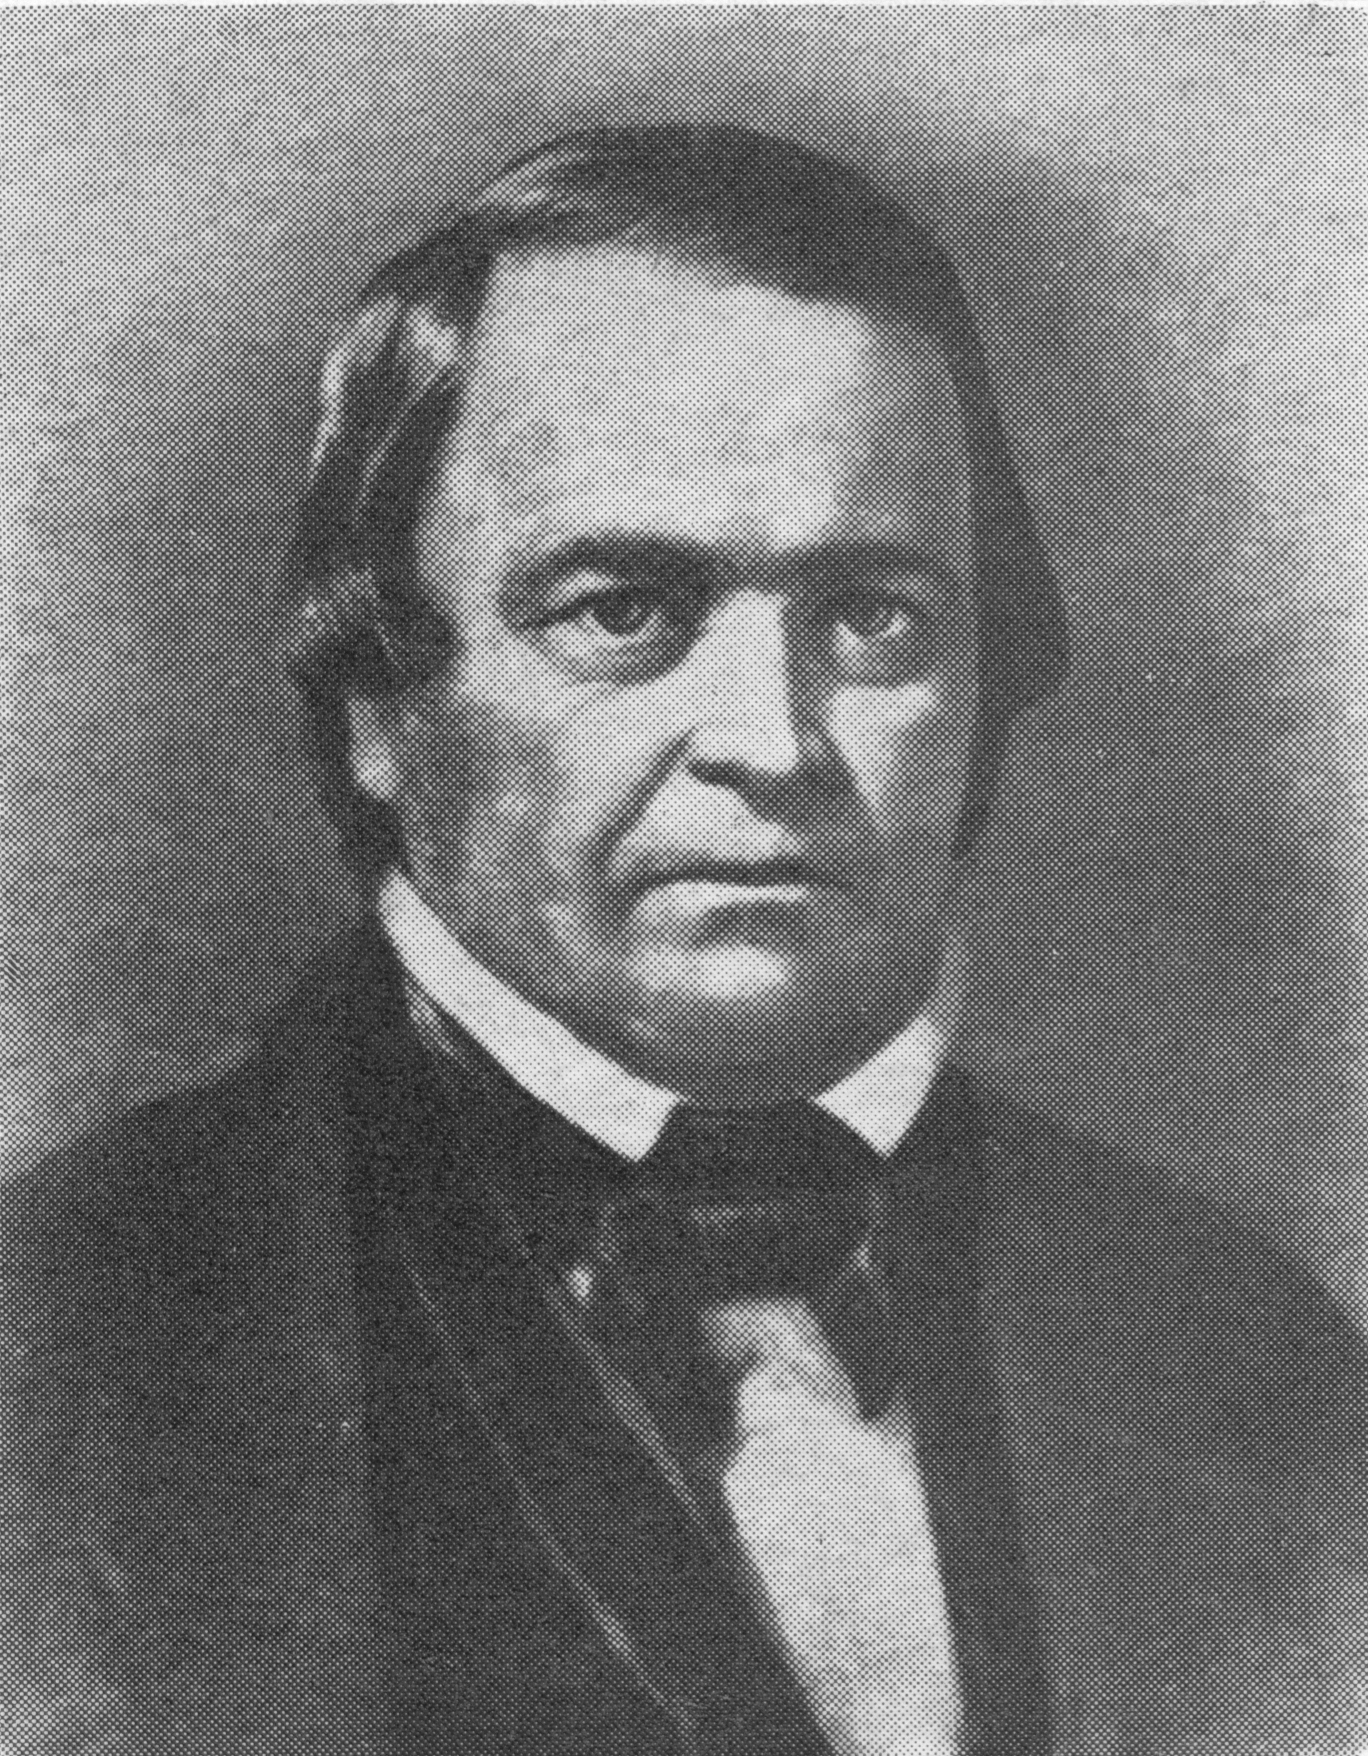
\includegraphics[width=1\linewidth]{images/william-miller.jpg}
    \caption*{William Miller (1782-1849)}
    \label{fig:w-miller}
\end{figure}


\begin{figure}[hp]
    \centering
    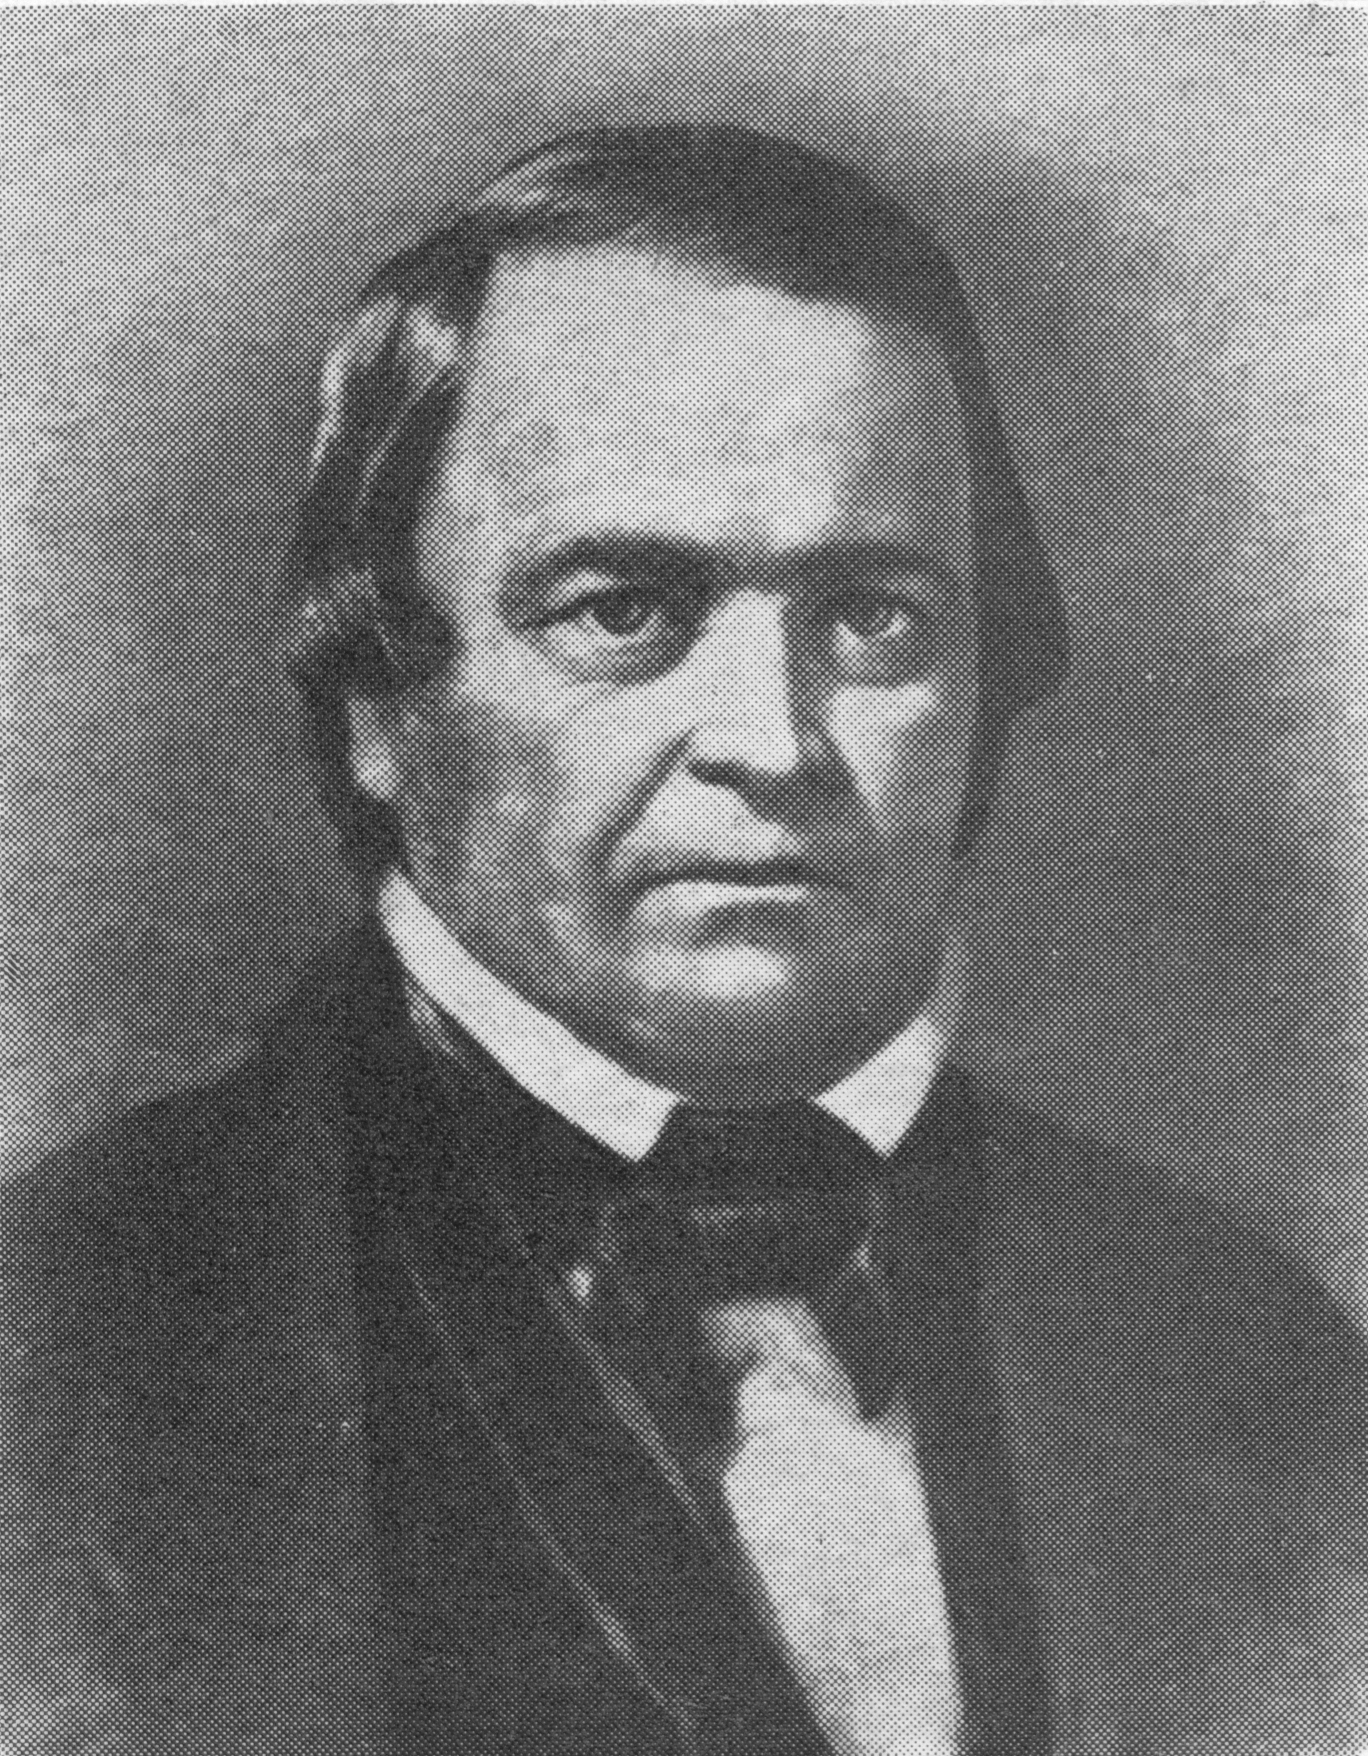
\includegraphics[width=1\linewidth]{images/william-miller.jpg}
    \caption*{ويليام ميلر (1782-1849)}
    \label{fig:w-miller}
\end{figure}


In reading the explanation of the great disappointment, did you see the answer to the question, “\textit{who is God whose judgment has come}?” The first angel’s message from Revelation 14:7 aligns exactly with the prophetic time declared in Daniel 8:14. The judgment that has come was the investigative judgment, which started in 1844. The Bible clearly describes whose hour of judgment has come in the first angel’s message. Let us read it in the Bible and see Ellen White’s comment.


عند قراءة تفسير خيبة الأمل العظيمة، هل رأيت الإجابة على السؤال، “\textit{من هو الله الذي جاءت ساعة دينونته}؟“ تتوافق رسالة الملاك الأول من رؤيا 14: 7 تمامًا مع الوقت النبوي المعلن في دانيال 8: 14. الدينونة التي جاءت كانت الدينونة التحقيقية، التي بدأت في عام 1844. يصف الكتاب المقدس بوضوح من جاءت ساعة دينونته في رسالة الملاك الأول. دعونا نقرأها في الكتاب المقدس ونرى تعليق إلين وايت.


\egw{‘I beheld,’ says the prophet Daniel, \textbf{‘till thrones were placed, and One that was \underline{Ancient of Days} \underline{did sit}}: \textbf{His raiment} was white as snow, and \textbf{the hair of His head} like pure wool; \textbf{His throne was fiery flames}, and the wheels thereof burning fire. A fiery stream issued and came forth from before Him: thousand thousands ministered unto Him, and ten thousand times ten thousand stood before Him: \textbf{\underline{the judgment was set, and the books were opened}}.’ Daniel 7:9, 10, R.V.}[GC 479.1; 1888][https://egwwritings.org/read?panels=p132.2169]


\egw{‘كنت أرى،‘ يقول النبي دانيال، \textbf{‘أنه وُضعت عروش، وجلس \underline{القديم الأيام}}: \textbf{لباسه} أبيض كالثلج، و\textbf{شعر رأسه} كالصوف النقي؛ \textbf{عرشه لهيب نار}، وعجلاته نار متقدة. نهر نار جرى وخرج من أمامه. ألوف ألوف تخدمه، وربوات ربوات وقوف قدامه. \textbf{\underline{جلس الدين، وفُتحت الأسفار}}.’ دانيال 7: 9، 10.}[GC 479.1; 1888][https://egwwritings.org/read?panels=p132.2169]


\egwnogap{\textbf{Thus was presented to the prophet’s vision the great and solemn day when the characters and the lives of men should pass in review before the Judge of all the earth, and to every man should be rendered ‘according to his works.’ \underline{The Ancient of Days is God the Father}.} Says the psalmist: \textbf{‘Before }the mountains were brought forth, or ever Thou hadst formed the earth and the world, even \textbf{from everlasting to everlasting}, \textbf{Thou art God}.’ Psalm 90:2. \textbf{\underline{It is He, the source of all being, and the fountain of all law, that is to preside in the judgment}}. And holy angels as ministers and witnesses, in number ‘ten thousand times ten thousand, and thousands of thousands,’ attend this great tribunal.}[GC 479.2; 1888][https://egwwritings.org/read?panels=p132.2170]


\egwnogap{\textbf{هكذا قُدم لرؤية النبي اليوم العظيم والمهيب الذي فيه ستمر شخصيات وحياة الناس في استعراض أمام ديان الأرض كلها، وسيُجازى كل إنسان ‘حسب أعماله’. \underline{القديم الأيام هو الله الآب}.} يقول المرنم: \textbf{‘قبل }أن تولد الجبال، أو أبدأت الأرض والمسكونة، \textbf{منذ الأزل إلى الأبد} \textbf{أنت الله}.’ مزمور 90: 2. \textbf{\underline{إنه هو، مصدر كل وجود، ونبع كل شريعة، الذي سيترأس في الدينونة}}. وملائكة قديسون كخدام وشهود، عددهم ‘ربوات ربوات، وألوف ألوف،‘ يحضرون هذه المحكمة العظيمة.}[GC 479.2; 1888][https://egwwritings.org/read?panels=p132.2170]


\egwnogap{\textbf{‘And, behold, one like \underline{the Son of man} came with the clouds of heaven, and came to \underline{the Ancient of Days}, and they \underline{brought Him near before Him}}. And there was given Him dominion, and glory, and a kingdom, that all people, nations, and languages, should serve Him: His dominion is an everlasting dominion, which shall not pass away.’ Daniel 7:13, 14. \textbf{The coming of Christ here described is not His second coming to the earth}. \textbf{\underline{He comes to the Ancient of Days in heaven} to receive dominion and glory and a kingdom}, \textbf{which will be given Him at the close of His work as a mediator}. \textbf{\underline{It is this coming, and not His second advent to the earth, that was foretold in prophecy to take place at the termination of the 2300 days in 1844}}. \textbf{Attended by heavenly angels, our great High Priest enters the holy of holies and there appears in \underline{the presence of God}} to engage in the last acts of His ministration in behalf of man—\textbf{to perform the work of investigative judgment} and to \textbf{make an atonement} for all who are shown to be entitled to its benefits.}[GC 479.3; 1888][https://egwwritings.org/read?panels=p132.2171]


\egwnogap{\textbf{‘وإذا مع سحب السماء مثل \underline{ابن إنسان} أتى وجاء إلى \underline{القديم الأيام}، \underline{فقربوه قدامه}}. فأُعطي سلطانًا ومجدًا وملكوتًا لتتعبد له كل الشعوب والأمم والألسنة. سلطانه سلطان أبدي ما لن يزول، وملكوته ما لا ينقرض.’ دانيال 7: 13، 14. \textbf{مجيء المسيح الموصوف هنا ليس مجيئه الثاني إلى الأرض}. \textbf{\underline{إنه يأتي إلى القديم الأيام في السماء} ليتسلم السلطان والمجد والملكوت}، \textbf{الذي سيُعطى له عند انتهاء عمله كوسيط}. \textbf{\underline{إنه هذا المجيء، وليس مجيئه الثاني إلى الأرض، الذي تنبأت به النبوة أنه سيحدث عند انتهاء الـ 2300 يوم في عام 1844}}. \textbf{محاطًا بملائكة سماويين، يدخل رئيس كهنتنا العظيم إلى قدس الأقداس ويظهر هناك في \underline{حضرة الله}} ليشارك في الأعمال الأخيرة من خدمته نيابة عن الإنسان—\textbf{ليقوم بعمل الدينونة التحقيقية} و\textbf{يقدم كفارة} لجميع الذين يتبين أنهم مستحقون لفوائدها.}[GC 479.3; 1888][https://egwwritings.org/read?panels=p132.2171]


The answer is simple and straightforward: The God of our pioneers was the Ancient of Days. \egwinline{The Ancient of Days is God the Father}. He is \textit{a personal}, \textit{spiritual being}. We see this in His description: \bible{Whose garment was white as snow, and the hair of his head like the pure wool: his throne was like the fiery flame, and his wheels as burning fire.}[Daniel 7:9]. In the termination of the 2300 days prophecy, in 1844, \bible{The hour of His judgment has come}[Revelation 14:7], \bible{the Ancient of days did sit} and \bible{the judgment was set, and the books were opened.}[Daniel 7:9,10]. The God from the first angel’s message is the Ancient of Days. Our pioneers were not ignorant regarding the truth about God. They believed \others{That there is \textbf{one God}, \textbf{\underline{a personal, spiritual being}}, \textbf{the creator of all things}, omnipotent, omniscient, and eternal, infinite in wisdom, holiness, justice, goodness, truth, and mercy; unchangeable, and \textbf{\underline{everywhere present by his representative, the Holy Spirit}}. Ps. 139:7.}[First point of the Fundamental Principles.] This one God is the Father, the Ancient of Days, \others{the creator of all things}, and we are to \bible{worship Him that made heaven, and earth, and the sea, and the fountains of waters}[Revelation 14:7]. He \bible{created all things by Jesus Christ}[Ephesians 3:9].


الإجابة بسيطة ومباشرة: إله روادنا كان القديم الأيام. \egwinline{القديم الأيام هو الله الآب}. إنه \textit{كائن شخصي}، \textit{روحي}. نرى هذا في وصفه: \bible{لباسه أبيض كالثلج، وشعر رأسه كالصوف النقي، وعرشه لهيب نار، وعجلاته نار متقدة.}[دانيال 7:9]. في نهاية نبوة الـ 2300 يوم، في عام 1844، \bible{قد جاءت ساعة دينونته}[رؤيا 14:7]، \bible{جلس القديم الأيام} و\bible{جلس الدين، وفُتحت الأسفار.}[دانيال 7:9،10]. الله في رسالة الملاك الأول هو القديم الأيام. لم يكن روادنا جاهلين بخصوص الحق عن الله. لقد آمنوا \others{أن هناك \textbf{إله واحد}، \textbf{\underline{كائن شخصي، روحي}}، \textbf{خالق كل الأشياء}، كلي القدرة، كلي العلم، وأبدي، لا نهائي في الحكمة، والقداسة، والعدل، والصلاح، والحق، والرحمة؛ لا يتغير، و\textbf{\underline{موجود في كل مكان بواسطة ممثله، الروح القدس}}. مز 139: 7.}[النقطة الأولى من المبادئ الأساسية.] هذا الإله الواحد هو الآب، القديم الأيام، \others{خالق كل الأشياء}، وعلينا أن \bible{نسجد للذي خلق السماء والأرض والبحر وينابيع المياه}[رؤيا 14:7]. هو \bible{خلق جميع الأشياء بيسوع المسيح}[أفسس 3:9].


Today, the first angel’s message has not lost any of its importance. The messages of the second and third angel’s depend on the first message and only the first message requires action on our part. We are to worship God. More specifically, we are to worship the right God. In the last and final conflict, there will be two kinds of worshippers, as we have been told in Revelation 13 and 14.


اليوم، لم تفقد رسالة الملاك الأول أيًا من أهميتها. تعتمد رسائل الملاك الثاني والثالث على الرسالة الأولى، والرسالة الأولى فقط هي التي تتطلب إجراءً من جانبنا. علينا أن نعبد الله. وبشكل أكثر تحديدًا، علينا أن نعبد الإله الصحيح. في الصراع الأخير والنهائي، سيكون هناك نوعان من العابدين، كما أُخبرنا في رؤيا 13 و14.


\bible{And all that dwell upon the earth shall \textbf{worship him} \normaltext{[the beast]}, \textbf{whose names are not written in the book of life of the Lamb} slain from the foundation of the world.}[Revelation 13:8]


\bible{فسيسجد له \textbf{جميع الساكنين على الأرض} \normaltext{[الوحش]}، \textbf{الذين ليست أسماؤهم مكتوبة في سفر حياة الخروف} المذبوح منذ تأسيس العالم.}[رؤيا 13:8]


The group that worships the beast will receive the mark of the beast. The whole world will be compelled to worship the beast and his image with the threat of death.


المجموعة التي تعبد الوحش ستتلقى سمة الوحش. سيُجبر العالم كله على عبادة الوحش وصورته تحت تهديد الموت.


\bible{And he \normaltext{[the beast]} had power to give life unto \textbf{the image of the beast}, that the image of the beast should both speak, and cause that \textbf{as many as would not worship the image of the beast should be killed}.}[Revelation 13:15]


\bible{وَأُعْطِيَ أَنْ يُعْطِيَ رُوحًا لِصُورَةِ الْوَحْشِ، حَتَّى تَتَكَلَّمَ صُورَةُ الْوَحْشِ، وَيَجْعَلَ \textbf{جَمِيعَ الَّذِينَ لاَ يَسْجُدُونَ لِصُورَةِ الْوَحْشِ يُقْتَلُونَ}.}[رؤيا ١٣: ١٥]


We should not participate in this worship. Let us learn and have faith just like Daniel’s three friends who refused to worship the image of King Nebuchadnezzar. The beast represented in Revelation 13, that extorts the consciences of men by the peril of their lives, is the papacy. Dear friend, don't be fooled. The papal God is a Trinity God. Do not overlook that.


يجب ألا نشارك في هذه العبادة. دعونا نتعلم ونتحلى بالإيمان مثل أصدقاء دانيال الثلاثة الذين رفضوا عبادة تمثال الملك نبوخذنصر. الوحش الممثل في رؤيا ١٣، الذي يبتز ضمائر الناس بخطر حياتهم، هو البابوية. عزيزي الصديق، لا تنخدع. إله البابوية هو إله الثالوث. لا تغفل عن ذلك.


We should worship the Ancient of Days as it is proclaimed in the first angel’s message. This is God the Creator who created everything through His Son, Jesus Christ. This is God from the first point of the \emcap{Fundamental Principles}. Our pioneers got this right.


يجب أن نعبد القديم الأيام كما هو معلن في رسالة الملاك الأول. هذا هو الله الخالق الذي خلق كل شيء من خلال ابنه، يسوع المسيح. هذا هو الله من النقطة الأولى من \emcap{المبادئ الأساسية}. لقد فهم روادنا هذا بشكل صحيح.


True understanding of the mission and purpose of the Seventh-day Adventist movement should be conclusive evidence that the Trinity doctrine is a foreign doctrine to us. We’ve ended up where we are today because we have forgotten \egwinline{\textbf{the way the Lord has led us, and \underline{His teaching} in our past history.}}[LS 196.2; 1915][https://egwwritings.org/read?panels=p41.1083] It is very sad to see how our Adventist scholars claim that our pioneers did not correctly understand the doctrine of God. If that were true, our pioneers would have failed to proclaim the first angel's message. They did not fail. We have failed.


إن الفهم الحقيقي لمهمة وهدف حركة الأدفنتست السبتيين يجب أن يكون دليلاً قاطعاً على أن عقيدة الثالوث هي عقيدة غريبة علينا. لقد انتهينا إلى ما نحن عليه اليوم لأننا نسينا \egwinline{\textbf{الطريقة التي قادنا بها الرب، و\underline{تعليمه} في تاريخنا الماضي.}}[LS 196.2; 1915][https://egwwritings.org/read?panels=p41.1083] من المحزن جداً أن نرى كيف يدعي علماؤنا الأدفنتست أن روادنا لم يفهموا عقيدة الله بشكل صحيح. لو كان ذلك صحيحاً، لفشل روادنا في إعلان رسالة الملاك الأول. لم يفشلوا. نحن الذين فشلنا.


\others{\textbf{Most of the founders of Seventh-day Adventism would not be able to join the church today if they had to subscribe to the denomination's Fundamental Beliefs}.}\others{\textbf{More specifically, most would not be able to agree to belief number 2, which deals with the doctrine of the Trinity.} For Joseph Bates the Trinity was an unscriptural doctrine, for James White it was that “old Trinitarian absurdity,” and for M. E. Cornell it was a fruit of the great apostasy, along with such false doctrines as Sunday-keeping and the immortality of the soul.}[George Night, Ministry Magazine, October 1993][https://www.ministrymagazine.org/archive/1993/10/adventists-and-change]


\others{\textbf{معظم مؤسسي الأدفنتست السبتيين لن يتمكنوا من الانضمام إلى الكنيسة اليوم إذا كان عليهم الالتزام بالمعتقدات الأساسية للطائفة}.}\others{\textbf{وبشكل أكثر تحديداً، معظمهم لن يتمكنوا من الموافقة على المعتقد رقم 2، الذي يتعامل مع عقيدة الثالوث.} بالنسبة لجوزيف بيتس كان الثالوث عقيدة غير كتابية، وبالنسبة لجيمس وايت كانت “سخافة الثالوث القديمة”، وبالنسبة لـ م. إي. كورنيل كانت ثمرة من ثمار الارتداد العظيم، إلى جانب عقائد خاطئة مثل حفظ الأحد وخلود الروح.}[جورج نايت، مجلة المنستري، أكتوبر 1993][https://www.ministrymagazine.org/archive/1993/10/adventists-and-change]


The doctrine of Trinity is the doctrine that undermines the foundation of our faith, the foundation that was laid at the beginning of our work. The distinction between truth and error lies in hermeneutics—the method of interpreting the Bible. Let us thoroughly investigate this issue.


عقيدة الثالوث هي العقيدة التي تقوض أساس إيماننا، الأساس الذي وُضع في بداية عملنا. الفرق بين الحق والخطأ يكمن في الهرمنيوطيقا - طريقة تفسير الكتاب المقدس. دعونا نحقق في هذه المسألة بشكل شامل.


\begin{titledpoem}
\stanza{
    In faith's first light, they sought His face, \\
    A vision pure, of divine grace. \\
    The pioneers, with vision clear, \\
    In 1844, held God so dear.
}

\stanza{    
    "The hour of judgment has come," they cried, \\
    To a world, both far and wide. \\
    The Ancient of Days, they did proclaim, \\
    Not a trinity, but a singular name.
}

\stanza{    
    Ellen White, with pen in hand, \\
    Spoke of a sanctuary, not of earthly land. \\
    A message of heaven, pure and bright, \\
    Guiding the faithful through the night.
}

\stanza{    
    The first angel’s message, a call to revere, \\
    God the Father, whom we should fear. \\
    "Who is the God we are to adore?" \\
    Not a trinity—this, they implored.
}

\stanza{    
    The Trinity, a concept unembraced, \\
    By pioneers, who in God's word traced. \\
    The Father, the Ancient, they did declare, \\
    His judgment and mercy, beyond compare.
}

\stanza{
    Yet, whispers now, through time have spread, \\ 
    A trinity's shadow, causing dread. \\
    If this be the God they were to declare, \\
    Their mission failed, caught in despair.
}

\stanza{
    But this is a falsehood, bold and cold, \\
    A narrative modern, but wrongly told. \\
    The Father they worshiped, with fervent zeal, \\
    Was the true God, their mission real.
}

\stanza{
    In unity, may we seek His face, \\
    Embracing truth, with grace and grace. \\
    The pioneers' vision, let us not lose, \\
    For in their footsteps, we must choose.
}

\stanza{
    To worship the God, of days of old, \\
    The Ancient of Days, as was foretold. \\
    In Revelation’s message, clear and bright, \\
    Guiding us still, through darkest night.
}
\end{titledpoem}